% ------------------------------------------------------------------------
% ------------------------------------------------------------------------
% ICMC: Modelo de Trabalho Acadêmico (tese de doutorado, dissertação de
% mestrado e trabalhos monográficos em geral) em conformidade com 
% ABNT NBR 14724:2011: Informação e documentação - Trabalhos acadêmicos -
% Apresentação
% ------------------------------------------------------------------------
% ------------------------------------------------------------------------

% Opções: 
%   Qualificação         = qualificacao 
%   Curso                = doutorado/mestrado
%   Situação do trabalho = pre-defesa/pos-defesa (exceto para qualificação)
% -- opções do pacote babel --
% Idioma padrão = brazil
	%spanish,			% idioma adicional para hifenização
	%english,			% idioma adicional para hifenização
	%brazil				% o último idioma é o principal do documento
\documentclass[qualificacao, mestrado, english, brazil]{packages/icmc}

% ---
% Pacotes Opcionais
% ---
\usepackage{rotating}           % Usado para rotacionar o texto
\usepackage[all,knot,arc,import,poly]{xy}   % Pacote para desenhos gráficos
% Este pacote pode conflitar com outros pacotes gráficos como o ``pictex''
% Então é necessário usar apenas um dos pacotes conflitantes

\newcommand{\VerbL}{0.52\textwidth}
\newcommand{\LatL}{0.42\textwidth}


% ---
% Informações de dados para CAPA e FOLHA DE ROSTO
% ---
% Tanto na capa quanto nas folhas de rosto apenas a primeira letra da primeira palavra (ou nomes próprios) devem estar em letra maiúscula, todas as demais devem ser em letra minúscula.
\tituloPT{Um editor de Ontologias Visual como ferramenta de apoio para a construção de sistemas inteligentes. }
%\tituloEN{A conceptual framework for the development of support systems for elderly}
\autor[Ribeiro, D. F.]{Douglas Francisco Ribeiro}
\genero{M} % Gênero do autor (M = Masculino / F = Feminino)
\orientador[Orientador]{Prof. Dr.}{Dilvan de Abreu Moreira}
%\coorientador{Prof. Dr.}{Fulano de Tal}
\curso{CCMC}
%\data{10}{8}{2016} % Data do depósito
% ---


% ---
% RESUMOS
% ---

% Resumo em PORTUGUÊS
% conter no máximo 500 palavras
% conter no mínimo 1 e no máximo 5 palavras-chave
\textoresumo[brazil]{

    A edição de ontologias, segundo \cite{Dragan2009} "o Protégé é a principal ferramenta de engenharia ontologica". Este software é desenvolvido na Universidade de Stanford e as versões anteriores foram desenvolvidos em colaboração com a Universidade de Manchester.
    
    A interface do Protégé fornece a possibilidade do usuário definir ontologias, ele inclui classificadores dedutivos para validar a consistencia dos modelos e para inferir novas informações com base na analise de uma ontologia. O grande problema neste processo é a necessidade de um conhecimento prévio do software, além de todo conhecimento sobre ontologia.
    
    O problema abordado na presente pesquisa é como desenvolver um sistema web para a exibição e edição de Ontologias, através da utilização das tecnologias da web semantica, para manter uma base conceitual adaptavel as mudanças do dominio, que de suporte ao armazenamento e à recuperação de informações.
    
    Alem dessa abordagem visual, será elaborada uma \sigla{DSL}{Domain Specific Language}, para satisfazer os requisitos dos Domain Experts. Neste caso, eles poderão digitar linhas de comandos ao invés de desenhar graficamente, e o software irá elaborar visualmente o mesmo.
    
    Os principais aportes do projeto são: diagramação visual, através de grafos e arvores, elaboração de comandos DSL para a criação de Ontologias por parte dos especialistas, e assim, fornecendo a flexibilidade necessária.
    
    }{Editor Visual, Ontologia, Ferramenta Apoio, Sistemas Inteligentes}


% resumo em INGLÊS
% conter no máximo 500 palavras
% conter no mínimo 1 e no máximo 5 palavras-chave
%\textoresumo[english]{
%
%    < escrever aqui >
%
%    }{Comprehensive Geriatric Assessment, Support system for the elderly, Rehabilitation %for elderly people}
    
% ---
% Configurações de aparência do PDF final
% ---
% alterando o aspecto da cor azul
\definecolor{blue}{RGB}{41,5,195}

% informações do PDF
\makeatletter
\hypersetup{
     	pagebackref=true,
		pdftitle={\@title}, 
		pdfauthor={\@author},
    	pdfsubject={\imprimirpreambulo},
	    pdfcreator={LaTeX with abnTeX2/ICMC-USP},
		pdfkeywords={\palavraschave}, 
		colorlinks=true,       		% false: boxed links; true: colored links
    	linkcolor=blue,          	% color of internal links
    	citecolor=blue,        		% color of links to bibliography
    	filecolor=magenta,      	% color of file links
		urlcolor=blue,
		bookmarksdepth=4
}
\makeatother
% --- 

% ----------------------------------------------------------
% ELEMENTOS PRÉ-TEXTUAIS
% ----------------------------------------------------------

% Inserir a ficha catalográfica
%\incluifichacatalografica*{tex/fichaCatalografica.pdf}
\incluifichacatalografica{634} % Código Cutter: número atribuído ao sobrenome do autor. Para obtê-lo, consulte a tabela Cutter Sanborn (em http://www.davignon.qc.ca/cutter1.html), procure pelo sobrenome ou forma mais próxima ao sobrenome completo e coloque o número indicado como parâmetro.


% DEDICATÓRIA / AGRADECIMENTO / EPÍGRAFE
%\textodedicatoria*{tex/pre-textual/dedicatoria}
%\textoagradecimentos*{tex/pre-textual/agradecimentos}
%\textoepigrafe*{tex/pre-textual/epigrafe}

% Inclui a lista de figuras
\incluilistadefiguras

% Inclui a lista de tabelas
\incluilistadetabelas

% Inclui a lista de quadros
%\incluilistadequadros

% Inclui a lista de algoritmos
%\incluilistadealgoritmos

% Inclui a lista de códigos
%\incluilistadecodigos

% Inclui a lista de siglas e abreviaturas
\incluilistadesiglas

% Inclui a lista de símbolos
%\incluilistadesimbolos

% ----
% Início do documento
% ----
\begin{document}
% ----------------------------------------------------------
% ELEMENTOS TEXTUAIS
% ----------------------------------------------------------
\textual

\chapter{Introdução}
\label{chapter:introducao}
\section{Contextualização}
\label{Contextualization}

A informação é matéria-prima para as organizações e as auxilia a sobreviver no mercado competitivo. A informação permite a interação entre diferentes departamentos e, também, possibilita aos gestores obter uma análise mais ampla da empresa. Cada indivíduo, no âmbito da organização, elabora um entendimento próprio sobre determinada informação, conforme afirma \cite{Choo2003} “a informação é fabricada por indivíduos a partir de sua experiência passada e de acordo com as exigências de determinada situação na qual a informação deve ser usada”.

As organizações estão começando a perceber a importância da informação. Atualmente, as pessoas em geral são expostas a uma grande quantidade de informação, sendo pressionadas a estar sempre bem informadas. Nesse contexto, torna-se necessário saber qual informação é relevante para determinada ação, seja simples ou complexa. Trata-se de uma questão de “inteligência”, ou seja, da habilidade para transformar a imensa massa de dados operacionais, que correm nas veias da empresa diariamente, em informações consistentes que agreguem valor ao negócio \cite{Teixeira2000}.

Dada a complexidade desses dados e como eles estão espalhados, faz-se necessário o uso de ferramentas que possam compreende-los automaticamente e, assim, apoiar tomadas de decisão mais rápidas e eficazes. Para compreender o significado em conjuntos de dados, programas necessitam associar informações semânticas a eles. Para isso, ontologias são usadas.

 Segundo Gruber (1995), uma ontologia é ”uma especificação explícita de uma conceitualização que representa o entendimento comum e a terminologia relevante de um domínio”. Ela é um sistema de organização e representação do conhecimento. Nesse contexto, Noy et al. (2001) relatam que as ontologias surgiram para compartilhar, organizar e especificar conhecimentos de um determinado domínio.
 
 Especialistas em um domínio de conhecimento, domain experts, são as pessoas indicadas para criar ontologias para esse domínio. Contudo, na maioria das vezes, esses especialistas não têm o domínio de ferramentas e linguagens para produzir ontologias que possam ser lidas por computadores.


\section{Motivação}

O tamanho e complexidade de ontologias cresce constantemente e as diversas origens dos usuários e áreas de aplicações multiplicam-se. Fornecer representações visuais e técnicas de interação intuitiva aos usuários pode ajudar significativamente a exploração e compreensão dos domínios representados por ontologias.

A Visualização/Edição de Ontologia não é um tema novo e um certo número de abordagens se tornaram disponíveis nos últimos anos. Algumas já estão bem estabelecidas, particularmente no campo da modelagem de ontologias. Em outras áreas da engenharia de ontologias, como alinhamento de ontologias e depuração, embora várias ferramentas tenham sido recentemente desenvolvidas, poucas fornecem uma interface gráfica do usuário, para não mencionar ajudas à navegação ou técnicas de visualização e interação abrangentes.

Na presença de uma enorme rede de recursos interligados na web, chamada de Linked Open Data (LOD), um dos desafios enfrentados pela comunidade é a visualização de conjuntos de dados multidimensionais para proporcionar uma visão geral eficiente. Com o foco passando de uma Web de documentos para uma Web de dados, mudanças nos paradigmas de interação estão em demanda também. Essas novas abordagens também precisam levar em consideração os desafios tecnológicos e oportunidades dadas por novos contextos de interação, por exemplo, toque e interação gestual.

Não há uma solução única, mas diferentes casos de uso que exigem diferentes técnicas de visualização e interação. Em última análise, proporcionando melhores interfaces de usuário, representações visuais e técnicas de interação irá promover o envolvimento dos usuários e, provavelmente, conduzem a resultados de maior qualidade em diferentes aplicações que empregam ontologias e assim, proliferar o consumo de dados vinculados.

Para que esta ferramenta possa ser desenvolvida, é importante identificar os requisitos que atendam às necessidades dos usuários, especialistas e das possíveis modelagens da Ontologia. Os estudos discutidos em \autoref {trabalhosrelacionados} não identificam quais requisitos foram utilizados para desenvolver ferramentas de sistema existentes. Assim, um quadro conceitual precisa ser desenvolvido com o objetivo de ajudar os desenvolvedores a criar ferramentas computacionais, a fim de apoiar os Domains Experts.

\section{Objetivos}

Com a finalidade de fornecer uma ferramenta de edição/visualização gráfica de Ontologias, que possa ser usada por domain experts, propõem-se, neste trabalho, o desenvolvimento de um sistema computacional, baseado na web, para a edição de ontologias.

A visualização gráfica, através de grafos e árvores, e a possibilidade do uso de comandos, numa linguagem próxima à usada por domain experts, vai permitir a criação/edição de ontologias por usuários fora da área da computação, com o mínimo de treinamento.

Este projeto de mestrado tem como objetivo propor e avaliar um editor de Ontologia Visual como ferramenta de apoio para construção de sistemas inteligentes, permitindo assim, que a partir de elementos visuais seje criado e/ou utilizada a Ontologia. O objetivo principal deste projeto pode ser dividido nos seguintes objetivos específicos:

\begin{itemize}
\item Permitir que o editor utilize Ontologias já criadas;
\item Permitir que se acrescente outras propriedades a Ontologias já criadas;
\item Criação de novas Ontologias para serem utilizadas;
\item Exportar os dados em formato compativel com \sigla{W3C}{World Wide Web Consortium} (\sigla{RDF}{Resource Description Framework} e/ou \sigla{OWL}{Web Ontology Language});
\end{itemize}

Para se estabelecer um quadro conceitual para o desenvolvimento do editor de Ontologia Visual, os requisitos devem ser identificados através da realização de uma revisão da literatura na área, e com entrevistas à especialistas. Posteriormente, esses requisitos recolhidos devem ser analisados e utilizados para construir os artefatos que compõem o quadro conceitual. Esses artefatos podem ser fluxos de trabalho, fluxogramas, diagramas de \sigla{UML}{Unified Modeling Language} ou \sigla{ERD}{Entity Relationship Diagram}. Para finalizar, é de suma importancia a construição de um protótipo para avaliar o quadro conceitual. Seguindo estes passos, é esperado que a todo o trabalho possa contribuir para o desenvolvimento de editor e que o mesmo possa estar apto a ser utilizado como elemento alternativo a escrita de Ontologias.

\section{Estrutura Proposta}

Esta tese de qualificação é organizada da seguinte forma: No capítulo 2 é apresentado os principais conceitos utilizados no desenvolvimento deste trabalho. No capítulo 3, os resultados do mapeamento sistemático são apresentados e no capítulo 4 é apresentado o trabalho proposto.

\chapter{Fundamentação Teórica}
\label{chapter:fundamentacao-teorica}
\label{fundamentacaoteorica}

\section{Web Semantica}
A web foi criada para possibilitar o acesso, intercâmbio e recuperação de informações de maneira rápida e simples, seu crescimento exponencial e caótico fez com que a mesma se tornasse hoje um gigantesco repositório de documentos, o que dificulta a recuperação de informações. Até o momento, não existe nenhuma estratégia abrangente e satisfatória para a indexação de documentos por meio de “motores de busca” que seja coerente com uma estrutura linguística. \cite{SouzaAlvarenga2004a} Com o intuito de preencher esse gargalo semântico na busca por informações, surge a web semântica. Ela tem como objetivo incorporar significado às informações presentes na web, criando um ambiente onde agentes de software e usuários possam trabalhar de forma cooperativa e entender o significado (sentido) presente nos dados. \cite{BrandaoLucena2002} Um exemplo da deficiência da web atual pode ser identificada na busca realizada pelos sistemas de recuperação de informação, que usam palavras-chave nas buscas,onde apenas a similaridade e o número de ocorrências de certas palavras no conteúdo de documentos são levados em consideração e não a semântica presente naquela informação. \cite{SouzaAlvarenga2004a}. 

Segundo a definição feita do W3C\footnote{http://www.w3.org/2001/sw}, a web semântica é um framework que permite compartir e reutilizar dados através das fronteiras das aplicações, empresas e comunidades. Ela tem duas funcionalidades principais: 

a) ser um conjunto de formatos para a integração e combinação de dados extraídos de diversas fontes, e; 

b) estabelecer uma linguagem para registrar como esses dados se referem a objetos do mundo real. 


\begin{figure}[!htb]
    \centering
    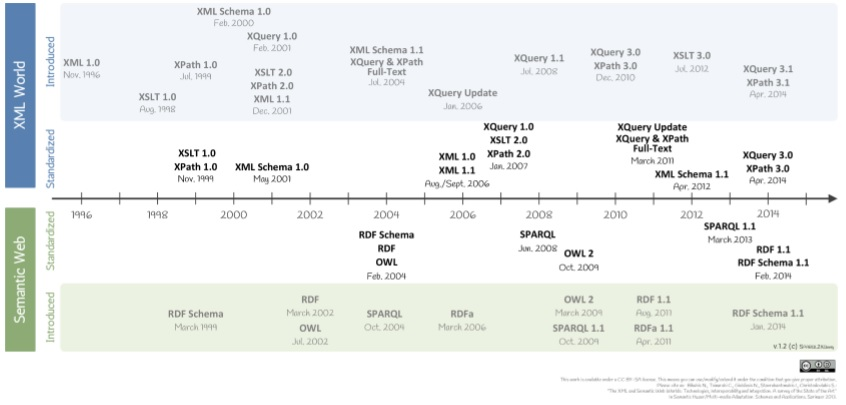
\includegraphics[width=12cm]{HistoriaWebSemantica.jpg}
    \caption{História da Web Semântica}
    \label{fig:HistoriaWebSemantica}
\end{figure}


A web semântica é formada por um conjunto de padrões propostos pelo World Wide Web Consortium (W3C). Eles evoluíram de padrões focados na representação de dados para a de conhecimento. Na \autoref{fig:HistoriaWebSemantica} podem ser observados os padrões que constituem a Web Semântica e sua relação com os padrões XML. Eles promovem formatos de dados comuns na WWW e também a inclusão de conteúdo Semântico na web, usando o padrão Resource Description Framework (RDF).

\section{Resource Description Framework}

O Resource Description Framework (RDF) é uma família de especificações da W3C, que foi disponibilizada em 1999 como parte do W3C Semantic Web Effort (Gruber, 1995). Ele foi originalmente projetado como um modelo de meta-dados e também chegou a ser usado como um método de descrições conceituais, principalmente para descrever recursos web. O RDF é usado em várias áreas de aplicação, como resource discovery para melhorar as capacidades dos motores de busca, cataloging para descrever o conteúdo e as relações de conteúdo disponibilizados em um sistema web particular, e descrição de intellectual property rights de páginas web. O modelo básico de dados consiste em um padrão de três tipos de objetos: 

\textbf{Sujeito:} representa os recursos e são identificados por meio de URIs, sem importar o tamanho deles, por exemplo, uma pagina web ou um elemento HTML podem ser recursos.

\textbf{Predicado:} são aspectos, características, atributos ou relações especificas que describem o sujeito, cada predicado têm um significado especifico e relaciona um sujeito com um objeto.

\textbf{Objeto:} um recurso especifico ou valor da propriedade que representa uma características do objeto\footnote{http://www.w3.org/TR/PR-rdf-syntax/}. 

Com RDF é possível explicitar relações entre dois objetos (usando-se uma Tripla RDF), mas não muito mais que isso. Para se descrever o que um objeto representa e suas relações com outros objetos, são necessárias ontologias.

\section{Ontologias}

A \autoref{fig:RepresentacaoOntologia} mostra os níveis de representação de dados na forma de conhecimento processável por máquinas.

\begin{figure}[!htb]
    \centering
    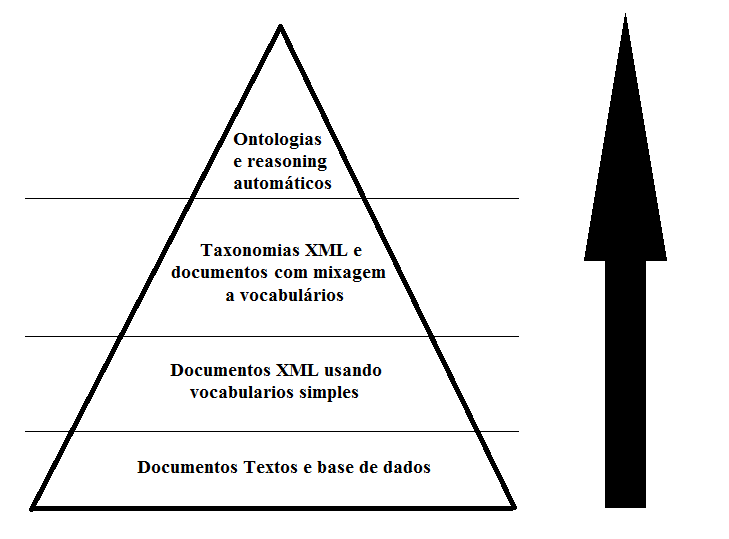
\includegraphics[width=12cm]{SmartDataContinuum.png}
    \caption{Níveis de Representação de Dados na forma de conhecimento processável por máquinas}
    \label{fig:RepresentacaoOntologia}
\end{figure}

O nível mais baixo de representação começa com os dados sem nenhum significado semântico, dependentes do contexto da aplicação. O segundo nível envolve a definição de esquemas XML para conseguir independência dos dados da aplicação, os dados fluem entre aplicações em um único domínio mas não podem ser compartilhados fora do domínio. No terceiro nível, os dados podem ser combinados a partir de diferentes domínios, sendo suficientemente independentes para serem recuperados e combinados com outras fontes de dados. Finalmente no quarto nível, é possível inferir novos dados a partir dos existentes e compartilha-los entre aplicações sem requerer interferência humana \cite{SugumaranGulla2011}, isso é possível graças as ontologias que descrevem esses dados. 

Uma ontologia é um sistema de organização e representação do conhecimento, em inglês \sigla{KOS}{Knowledge Organization System}, que é uma estrutura conceitual e computacional que permite representar o conhecimento, de qualquer domínio, por meio de entidades, classificações, relações semânticas, regras e axiomas.

Contudo, não existe um consenso sobre uma exata definição para ontologias. Segundo \cite{Gruber1995}, uma ontologia é "uma especificação explícita de uma conceitualização que representa o entendimento comum e a terminologia relevante de um domínio".

Uma ontologia é especificada por meio de componentes básicos que são as classes, relações, axiomas e instâncias. As classes, o foco da maioria das ontologias, são utilizadas para descrever os conceitos de um domínio, possibilitando a organização das classes em um sistema lógico e hierárquico contendo subclasses que representam conceitos mais específicos \cite{Noy2001}. As relações representam o tipo de interação entre os conceitos de um domínio e as propriedades presentes nas classes e indivíduos. Elas podem ter características próprias, como serem transitivas, simétricas, ou terem uma cardinalidade definida. Os axiomas são utilizados para modelar regras assumidas como verdadeiras no domínio em questão, de modo que seja possível associar o relacionamento entre os indivíduos, além de fornecer características descritivas e lógicas para os conceitos. Para \cite{UscholdGruninger1996} os axiomas são especificados para definir a semântica e significado dos termos (classes e propriedades) e sugerem que a fase de definição dos axiomas (especificação da ontologia) é a mais difícil na construção de ontologias. Por fim, os indivíduos, ou instâncias das classes, são utilizados para representar elementos específicos, ou seja, os próprios dados, que, juntamente com a definição de uma ontologia, constituem a base de conhecimento \cite{Noy2001}.


\section{Web Ontology Language}

A Web Ontology Language (OWL) foi recomendada pelo W3C em 2004 para representar e compartilhar ontologias na Web. Essa linguagem foi projetada para aplicações que necessitam processar o conteúdo da informação em vez de apenas apresentar informações em nós \cite{McGuinness2004}. OWL é uma linguagem que permite que semântica seja explicitamente associada ao conteúdo dos dados na web e formalmente especificada através de ontologias, compartilhadas na Internet.

A OWL 2, de abril de 2008, é a versão mais recente da linguagem 2. De acordo com as especificações do W3C\footnote{http://www.w3.org/TR/owl2-overview}, a OWL 2 adicionou três novos perfis (sub-linguagens) aos perfis DL e Full já existentes: OWL 2 EL, OWL 2 QL e OWL RL (\autoref{fig:OWLProfile}). Cada um desses perfis oferece um poder de expressividade diferente para diversos cenários de aplicação:

\begin{itemize}
    \item \textbf{FULL}: É direcionado para usuários que querem a máxima expressividade e a liberdade sintática do RDF sem nenhuma garantia computacional. É improvável que qualquer software de raciocínio seja capaz de suportar completamente cada recurso da OWL Full \cite{McGuinness2004}.

    \item \textbf{DL}: (Description Logic) é para aplicações que necessitam de máxima expressividade, enquanto mantém a computabilidade (todas as conclusões são garantidos para ser computáveis) e decidibilidade (todas as computações terminarão em tempo finito) \cite{McGuinness2004}. O OWL DL inclui todas as construções da linguagem OWL, mas elas podem ser usadas somente sob certas restrições.

    \item \textbf{EL}: É baseado na família EL++ de lógica descritiva (Description Logic), esse perfil é particularmente útil em aplicações utilizando ontologias que contêm um grande número de propriedades e/ou classes. Além disso, o OWL 2 EL utiliza um padrão comum utilizado em ontologias para conceitos e planejamento, ou seja, a combinação de conjunção e qualidades existenciais.

    \item \textbf{QL}: É baseado na família DL-Lite de lógica descritiva. Esse perfil foi criado para permitir o raciocínio (reasoning) eficiente com grandes quantidades de dados estruturados de acordo com esquemas relativamente simples. Ele fornece a maioria dos recursos necessários para capturar modelos conceituais, tais como diagramas de classe UML, diagramas de Entidade de Relacionamento, e esquemas de banco de dados.
 
    \item \textbf{RL}: É voltado para aplicações que exigem raciocínio escalável em troca de alguma restrição de poder expressivo. Ele define um subconjunto sintático de OWL 2 que favorece a implementação utilizando tecnologias baseadas em regras. Esse perfil pode ser utilizado na maioria das construções OWL 2, porém, para permitir implementações baseadas em regras de raciocínio, a forma como essas construções podem ser usadas em axiomas foi restringida.

\end{itemize}

\begin{figure}
    \centering
    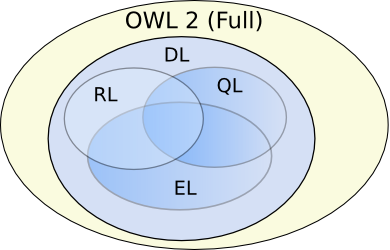
\includegraphics[width=12cm]{Owl2-profiles.png}
    \caption{OWL 2 Profiles}
    \label{fig:OWLProfile}
\end{figure}

Em um Sistema de Apoio a Decisão (SAD), ontologias podem ser usadas para modelar o domínio da aplicação deste sistema.


\chapter{Trabalhos Relacionados}
\label{chapter:trabalhos-relacionados}
\label{trabalhosrelacionados}

Após uma pesquisa bibliográfica foi possivel constatar que existem varios software que se propoem a trabalhar com Ontologias, e foi encontrado somente um software com a capacidade de visualização dessas ontologias em formato de grafos.

\section{Protégé}

\begin{figure}[h]
    \centering
    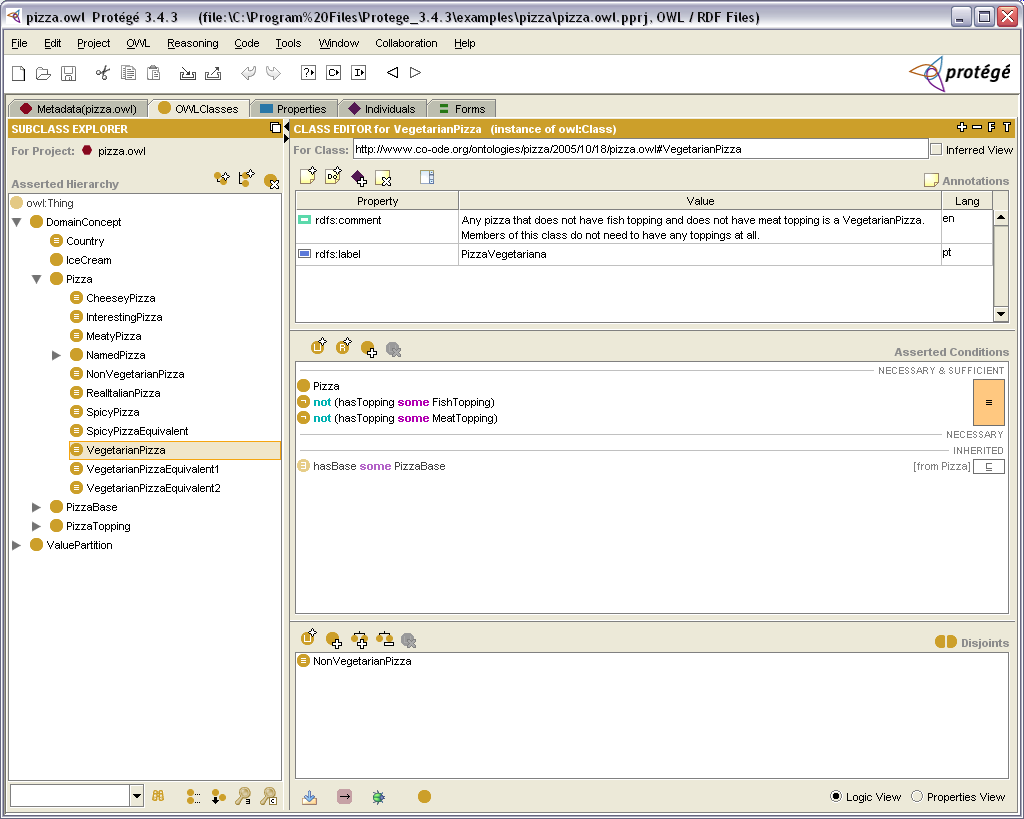
\includegraphics[width=12cm]{Protege_3.png}
    \caption{Tela Principal do Software Protégé}
    \label{fig:Protege343}
\end{figure}

O Protégé\footnote{http://protege.stanford.edu/products.php} é um software livre (opensource), com estrutura para a construção de sistemas inteligentes.

Sua interface é baseada em formularios (\autoref{fig:Protege343}), e portanto mais complexa de se trabalhar. Apesar da interface necessitar de um conhecimento mais aprimorado, os recursos oferecidos pelo Protégé não são encontrados em outros softwares.

Para poder utilizar esta ferramenta, é necessário sua instalação no computador.

\section{WebVOWL}
O VOWL\footnote{http://www.http://vowl.visualdataweb.org/} é uma linguagem visual bem especificada para a representação orientada para o utilizador de ontologias. Ele define representações gráficas para a maioria dos elementos do Web Ontology Language (OWL), que são combinados para um layout gráfico direcionado, visualizando a ontologia (\autoref{fig:WebVOWL}). Em contraste com trabalhos relacionados, VOWL aponta para uma representação intuitiva e abrangente que também é compreensível para os usuários menos familiarizados com ontologias. Ele é um aplicativo independente inteiramente baseado em padrões web abertos. 


\begin{figure}[h]
    \centering
    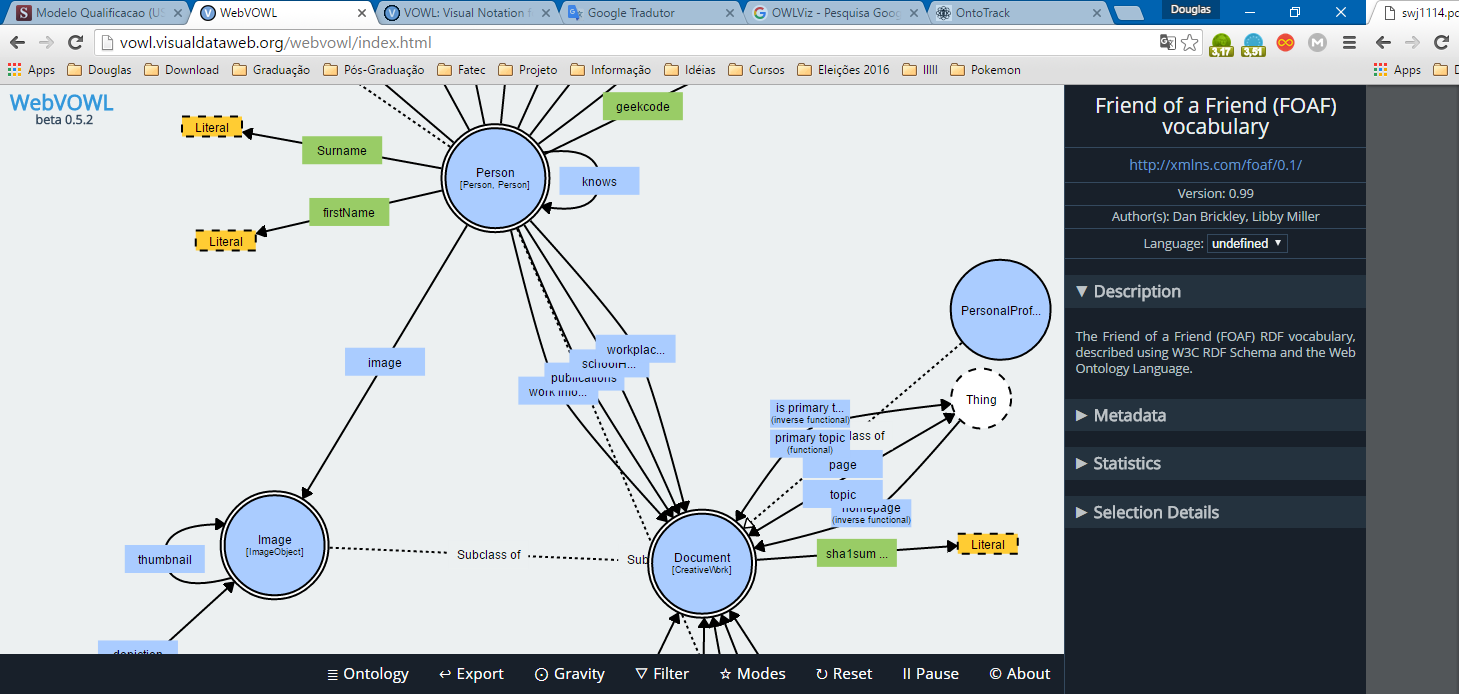
\includegraphics[width=12cm]{WebVOWL.png}
    \caption{Tela Principal do Software WebVOWL}
    \label{fig:WebVOWL}
\end{figure}

O VOWL serve unicamente como visualizador de ontologia em formato de grafos, não sendo possivel sua edição. Outra situação, no VOWL é que também não é possivel a resolução da ontologia (RESORNER), pois o mesmo não tem tal recurso.

\section{OntoTrack}

Na \autoref{fig:OntoTrack}, é demonstrada a interface do software OntoTrack. Como pode-se observar ele não é web e portanto existe a necessidade de se instalar o aplicativo no computador. Outra caracteristica é que apesar da instalação, existem versões para os sistemas operacionais mais utilizados hoje (Windows, Linux, MacOS e SunOS). Após instalado ele ira ocupar aproximadamente 8 mb de espaço, o que não tem um peso muito grande nos equipamentos atuais.

A importação de arquivos para o OntoTrack assim como a exportação, usa o parser RDF Jena2 \cite{McBride2001}. O modelo de ontologia interna da Jena2 de classes e propriedades também serve como modelo de representação central para o OntoTrack. Atualmente, OntoTrack é capaz de ler e escrever ontologias OWL Lite. No entanto, as propriedades, bem como propriedade global, restrições (declarações de domínio e alcance) não são editáveis no OntoTrack no momento.

\begin{figure}[h]
    \centering
    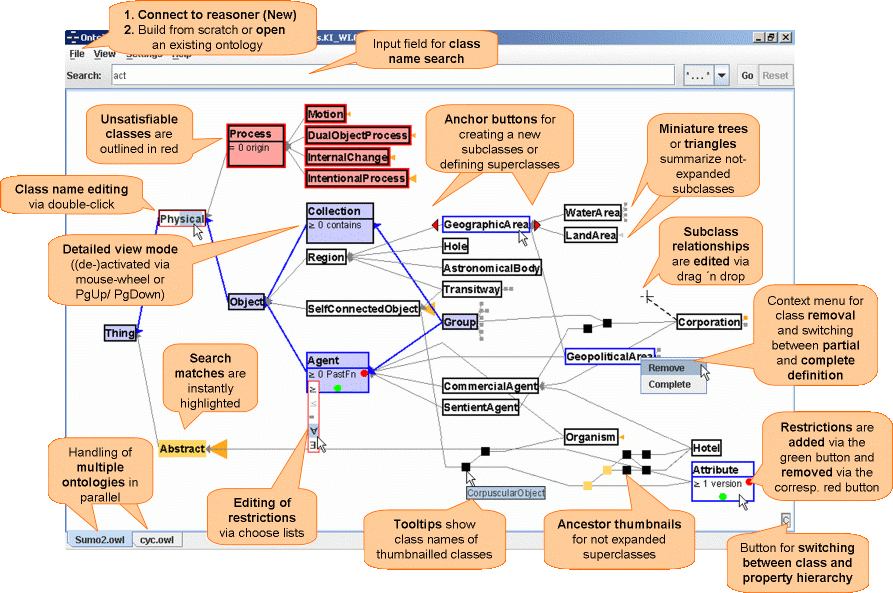
\includegraphics[width=12cm]{OnTrack.png}
    \caption{Tela Principal do Software OntoTrack}
    \label{fig:OntoTrack}
\end{figure}


\section{OWLViz}

O OWLViz é projetado para ser usado com o editor Protege-OWL. Ele permite hierarquias de classe em uma Ontologia OWL para ser visto e incrementalmente navegado, permitindo a comparação da hierarquia de classes afirmada e a hierarquia de classe inferida. O OWLViz integra com o editor Protege-OWL, utilizando o mesmo esquema de cores de modo que as classes primitivas e definidas podem ser distinguidos, mudanças computados para a hierarquia de classes pode ser visto claramente, e os conceitos inconsistentes são destacadas em vermelho, tem a facilidade para salvar ambos os pontos de vista afirmados e inferidos da hierarquia de classes para vários formatos gráficos, incluindo PNG, JPEG, e SVG.

Na \autoref{fig:OwlViz} pode ser visto a tela principal do Protege-OWL com o uso do plugin OWLViz. Assim como o Protégé, é necessário a instalação deste plugin no computador, alem disse, tem que se observar a versão do plugin se é compativel com a versão do Protégé instalada. Caso faça atualização no software Protégé, este plugin terá que ser atualizado também.

\begin{figure}[h]
    \centering
    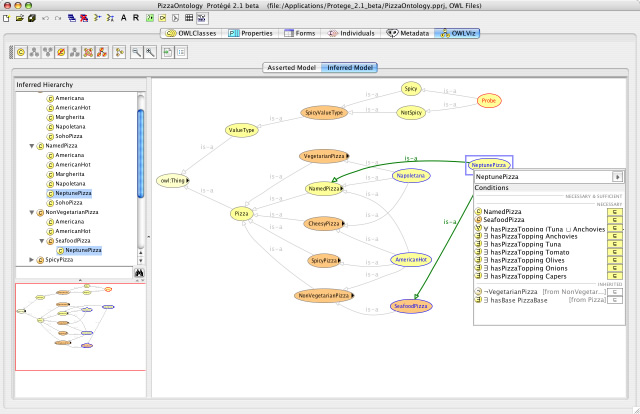
\includegraphics[width=12cm]{OwlViz.jpg}
    \caption{Tela Principal do Software Protégé com o Plugin OWLViz}
    \label{fig:OwlViz}
\end{figure}


\section{Conciderações Finais}

Apesar de existir ferramentas para elaboração de ontologias e para sua visualização em formato de grafos, não foi localizado nenhuma ferramenta que tenha suporte satisfatório aos dois tipos, podendo inclusive mudar a visualização de acordo com o especialista que trabalho com o sistema.

\chapter{Proposta de Trabalho}
\label{chapter:proposta-trabalho}
\section{Plano de Trabalho}

Neste capítulo será descrito o plano de trabalho que está guiando o desenvolvimento do presente projeto.

\subsection{Metodologia}
\label{development_methodology}

Nesta seção será descrita a metodologia de desenvolvimento deste projeto. Ela é divida em dois métodos de desenvolvimento principais: para as ontologias e para o sistema web que suportará o processo de edição/visualização.

\subsection{Ontologias}

O conhecimento do domínio envolvido em Linked Data está em contínua ampliação, por este motivo faz necessário um enfoque na possibilidade de mudança na estrutura de exibição das Ontologias. Sua capacidade de representar o conhecimento de um domínio por meio de formatos, como a linguagem OWL, permiti separar o conhecimento das outras partes do sistema. Os modelos OWL permitem a compilação do conhecimento em sistemas de armazenamento e recuperação de informação, chamados triplestores, que são bancos de dados e que adicionam significado semântico aos seus dados. Neste sistema será apresentado a visualização e interação de Ontologias e Linked Data.

\subsection{Sistema Web}

Os componentes da arquitetura do sistema web são parte deste trabalho (interface gráfica) e parte de um outro trabalho de mestrado. A ideia é construir um software que possa ser reusados em outros \sigla{SAD}{Sistemas de Apoio a Decisão}, tendo ou não similaridade com esta pesquisa.

\subsubsection{Groovy}
O desenvolvimento do software será feito usando-se uma DSL baseada na linguagem Groovy \cite{Koenigetal2007}. Ou seja, essa DSL será uma extensão da linguagem Groovy. Groovy é uma linguagem que tem suporte ao desenvolvimento de DSLs. Isso inclui suporte a DSL Descriptors, arquivos Groovy que descrevem extensões domain-specific para o motor de inferência e assistente de conteúdo do plugin Groovy-Eclipse. Isso permite que a DSL criada tenha todo o suporte que o IDE Eclipse dá a linguagens como Java ou Groovy, como code completion, debugging, etc. Uma outra vantagem de Groovy é a disponibilidade do Grails Framework para a criação de aplicações Web \cite{Judd2008}. O uso da DSL por especialistas em diversas areas e a utilização em conjunto com um SAD, deve permitir o seu aprimoramento.

\subsubsection{Canvas e SVG} 
Uma análise de tecnologias de gráficos vetoriais disponíveis nos últimos navegadores modernos, mostra que novos cenários podem ser criados usando tecnologias padrão da Web de uma forma interativa. Pensando nesse requisito foi feito um levantamento de caracteristicas entre duas técnologias bastante interessantes.

O \sigla{SVG}{Scalable Vector Graphics} é conhecido como um modelo de elementos gráficos de modo retido persistindo em um modelo na memória. Análogo ao HTML, o SVG cria um modelo de objeto de elementos, atributos e estilos. Quando o elemento <svg> aparece em um documento HTML5, ele se comporta como um bloco alinhado e faz parte da árvore do documento HTML \cite{PatrickDengler2013}.

O \sigla{Canvas}{Elemento HTML} é um bitmap com uma interface de programação de aplicativo (API) de elementos gráficos de modo imediato para desenhar. O Canvas é um modelo "dispare e esqueça" que renderiza os elementos gráficos diretamente em seu bitmap e depois, subsequentemente, não tem nenhuma noção das formas desenhadas; apenas o bitmap resultante permanece \cite{PatrickDengler2013}.

Uma forma de pensar nisso é que o Canvas lembra a API Windows GDI, em que você desenha elementos gráficos programaticamente em uma janela e o SVG lembra marcação HTML com elementos, estilos, eventos e capacidade de programação baseada no DOM. O Canvas é procedimental, enquanto o SVG é declarativo.

Na \autoref{tab:ComparacaoCanvasSVG} é demonstrado uma comparação entre Canvas e SVG.

\begin{table}[h!]
    \centering
    \caption{Comparação Canvas x SVG}
    \label{tab:ComparacaoCanvasSVG}
    \begin{tabular}{|c|c|} \hline
        Canvas &  SVG & \hline
        Baseado em pixel (o canvas é essencialmente um elemento de imagem com uma API de desenho) & 
        Baseado em modelo de objeto (elementos do SVG são similares a elementos HTML) & \hline
        Elemento HTML único similar a <img> no comportamento & Múltiplos elementos gráficos que se tornam parte do Modelo de objeto de documento (DOM) & \hline
        Apresentação visual criada e modificada programaticamente através de script & 
        Apresentação visual criada com marcação e modificada por CSS ou programaticamente através de script & \hline
        A interação modelo de evento/usuário não é refinada — apenas no elemento canvas; interações devem ser programadas manualmente a  partir de coordenadas do mouse &
        A interação modelo de evento/usuário é baseada em objeto no nível de elementos gráficos primitivos — linhas, retângulos, caminhos &
    \end{tabular}
\end{table}

\subsection{Desenvolvimento}
Será necessário a aplicação de alguma metodologia de desenvolvimento de software. Neste cenário, existem vários métodos e metodologias que permitem um desenvolvimento ágil de software. Nesse contexto, o termo ágil refere-se ao desenvolvimento em tempos curtos e geração de protótipos facilmente adaptáveis às mudanças. Exemplos de métodos ágeis são: “Mockups”, “User Stories”, “Scenarios”, “Storyboards” e “Use Cases”, exemplos de metodologias ágeis são: “SCRUM” ou “XP eXtreme Programming”.

Uma das etapas mais importantes dos desenvolvimentos ágeis é o levantamento de requisitos. Essa etapa tem como objetivo definir as características do software e pode ser realizada múltiplas vezes. Isso ocorre pois as metodologias ágeis são cíclicas e os protótipos mudam em  cada ciclo para cumprir os requisitos. O deste sistema será realizado por meio de metodologias ágeis de desenvolvimento de software, principalmente serão utilizadas algumas práticas da metodologia SCRUM \cite{SchwaberBeedle2002}. Também será usado o enfoque UserCentered Design. Nesse sentido, está sendo desenvolvido primeiramente um mockup da interface gráfica do sistema, o qual será o meio de interação com os usuários para a elaboração das Ontologias. Quando o mockup for validado, será iniciado o desenvolvimento de um protótipo da interface gráfica que permitirá determinar os requisitos funcionais. 

\subsection{Atividades Previstas e Cronograma}

A seguir, são descritas as principais atividades a serem realizadas para o desenvolvimento deste trabalho, visando cumprir os objetivos e tendo como referência a metodologia proposta. A duração de cada uma das atividades está descrita no cronograma de atividades \autoref{tab:atividades}. As seguintes atividades foram previstas para ter início em Agosto de 2015 e duração de 24 meses: 

\begin{itemize}
  \label{tab:atividades}
  \item \textbf{A1}- Obtenção de créditos referente as disciplinas do programa de mestrado.
  \item \textbf{A2}- Exame de Proficiência na língua inglesa.
  \item \textbf{A3}- Levantamento bibliográfico sobre a área de pesquisa.
  \item \textbf{A4}- Estudo sobre Web Semântica.
  \item \textbf{A5}- Estudo sobre Ontologias.
  \item \textbf{A6}- Desenvolvimento da ontologia do software.
  \item \textbf{A7}- Desenvolvimento dos controles visuais.
  \item \textbf{A8}- Qualificação: redação da monografia de qualificação.
  \item \textbf{A9}- Exame de Qualificação.
  \item \textbf{A10}- Implementação do primeiro protótipo.
  \item \textbf{A11}- Testes preliminares, refinamento e reimplementação.
  \item \textbf{A12}- Testes e validação: estudos de casos e refinamentos.
  \item \textbf{A13}- Redação da Dissertação.
  \item \textbf{A14}- Redação e submissão de artigos com os resultados obtidos.
  \item \textbf{A15}- Defesa.

\end{itemize}

A \autoref{tab:cronograma} apresenta o cronograma de execução das atividades.

\begin{table}[h!]
    \centering
    \caption{Cronograma do projeto}
    \label{tab:cronograma}
    \begin{tabular}{|c|c|c|c|c|c|c|c|c|} \hline
        Ativ. &
        \multicolumn{2}{|c|}{2015} &
        \multicolumn{4}{|c|}{2016} &
        \multicolumn{2}{|c|}{2017} \\ \hline
               &
         3 Tri &
         4 Tri &
         1 Tri &
         2 Tri &
         3 Tri &
         4 Tri &
         1 Tri &
         2 Tri \\ \hline
         A1 & . & ... & ... & ... & ... & ... & & \\ \hline
         A2 & & ... & ... & ... & ... & & & \\ \hline
         A3 & & & ... & ... & ... & ... & & \\ \hline
         A4 & & & ... & ... & ... & ... & & \\ \hline
         A5 & & & .. & ... & ... & ... & & \\ \hline
         A6 & & & & . & .. & ... & & \\ \hline
         A7 & & & & . & .. & ... & & \\ \hline
         A8 & & & & & ... & & & \\ \hline
         A9 & & & & & & ... & & \\ \hline
         A10 & & & & & & .. & & \\ \hline
         A11 & & & & & & .. & ... & ... \\ \hline
         A12 & & & & & & .. & ... & ... \\ \hline
         A13 & & & & & & ... & ... & ...\\ \hline
         A14 & & & & & & ... & & ...\\ \hline
         A15 & & & & & & & & . \\ \hline
         
    \end{tabular}
\end{table}

\subsection{Atividades Concluídas até o Momento}

No cronograma, todas as atividades de A1 a A7 estão sendo concluídas. Além disso, a redação e submissão de artigos com os resultados obtidos, estão sendo realizadas.

\section{Dificuldades e Limitações}

Em virtude de minha formação como tecnologo, tive muita dificuldade no inicio, tendo que pesquisar constantemente com referência a varios assuntos ligados a pesquisa.

Varias das linguagens abordadas não era de meu conhecimento e esse processo de aprendizado foi mais despendioso do que o inicialmente planejado, além é claro, da falta de tempo dispendido para isso, pois tenho emprego fixo e isso acabou gerando uma dificuldade maior.

Tirando esses pequenos impedimentos iniciais, o processo esta sendo desenvolvido de forma bem elaborada, dentro do cronograma elaborado.



% ---
% Finaliza a parte no bookmark do PDF, para que se inicie o bookmark na raiz
% ---
\bookmarksetup{startatroot}% 
% ---

% ----------------------------------------------------------
% ELEMENTOS PÓS-TEXTUAIS
% ----------------------------------------------------------
\postextual

% ----------------------------------------------------------
% Referências bibliográficas
% ----------------------------------------------------------


\bibliography{referencias}

% ---------------------------------------------------------------------
% GLOSSÁRIO
% ---------------------------------------------------------------------

% Arquivo que contém as definições que vão aparecer no glossário

\newword{Framework}{É uma abstração que une código comum entre vários projetos de software que fornecem uma funcionalidade genérica. Frameworks são concebidos com a intenção de facilitar o desenvolvimento de software, permitindo que designers e desenvolvedores de passar mais tempo na determinação dos requisitos de software do que com detalhes de baixo nível do sistema. Software Framework compreende um conjunto de classes implementadas em uma linguagem de programação específica utilizada para apoiar o desenvolvimento de software.}

\newword{Framework Conceitual}{A estrutura teórica de pressupostos, princípios e regras que une as idéias que compreende um conceito amplo. Framework Conceitual, não é um software executável, mas um modelo de dados para um domínio.}

\newword{Artifact}{É o produto de uma ou mais atividades dentro do contexto de um desenvolvimento de software. Assim, cada fase / iteração do desenvolvimento irá resultar em um documento (por exemplo fluxograma, DER, fluxo de trabalho, diagramas UML ou qualquer outro documento) que servirá como uma fonte de informação.}


\newword{Tecnologia Assistiva}{Ele refere-se a produtos, recursos, metodologias, estratégias, práticas e serviços que visam promover a funcionalidade de pessoas com deficiência, deficiência ou mobilidade reduzida, por sua autonomia, independência, qualidade de vida e inclusão social.}

\newword{Realidade Virtual}{É uma tecnologia de interface avançada entre um usuário e um sistema de computador. O objetivo desta tecnologia é recriar ao máximo a sensação de realidade para um indivíduo. Portanto, essa interação acontece em tempo real, utilizando técnicas e equipamentos computacionais para auxiliar na expansão do sentimento de presença do usuário.}

\newword{Webservices}{É uma solução usada em sistemas de integração e comunicação entre diferentes aplicações. Com esta tecnologia é possível que novas aplicações possam interagir com as que já existam e que sistemas desenvolvidos em diferentes plataformas sejam compatíveis.}
% Comando para incluir todas as definições do arquivo glossario.tex
\glsaddall
% Impressão do glossário
% \printglossaries

% ----------------------------------------------------------
% Apêndices
% ----------------------------------------------------------

% ---
% Inicia os apêndices
% ---
%\begin{apendicesenv}
%
%   \chapter{Entity Relationship Diagram (ERD)}
%    \label{chapter:erd}
%    The entities compose the Entity Relationship Diagram (ERD) to develop a dynamic form for CGA and available on the web is present in \autoref{fig:der_cga}.

\begin{figure}[htb]
\caption{ERD proposed for CGA Web}
 \label{fig:der_cga}
 \centering
 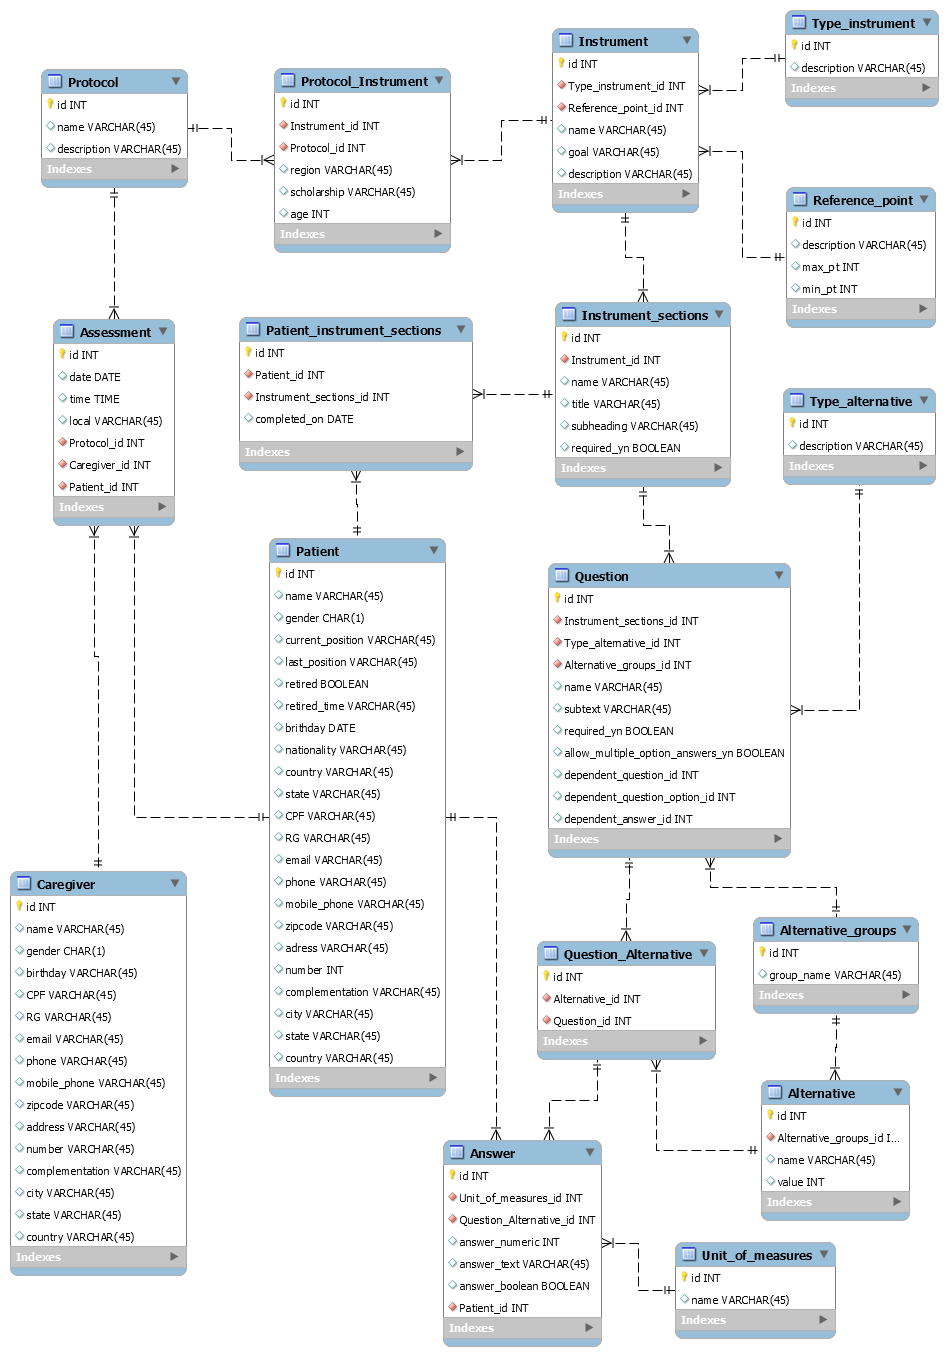
\includegraphics[scale=0.27]{der_cga.png}
 \fautor
\end{figure}

%    
%    \chapter{Timed Up and Go Test (TUG)}
%    \label{chapter:tug-kinect}
%    The "Timed Up and Go Test" (TUG) was developed to compose the Kinect application. The \autoref{fig:img_1_kinect}, \autoref{fig:img_1e2_kinect} and \autoref{fig:img_3_kinect} present the screens of the Kinect application developed.

\begin{figure}[htb]
\caption{Start screen of TUG assessment using Kinect}
 \label{fig:img_1_kinect}
 \centering
 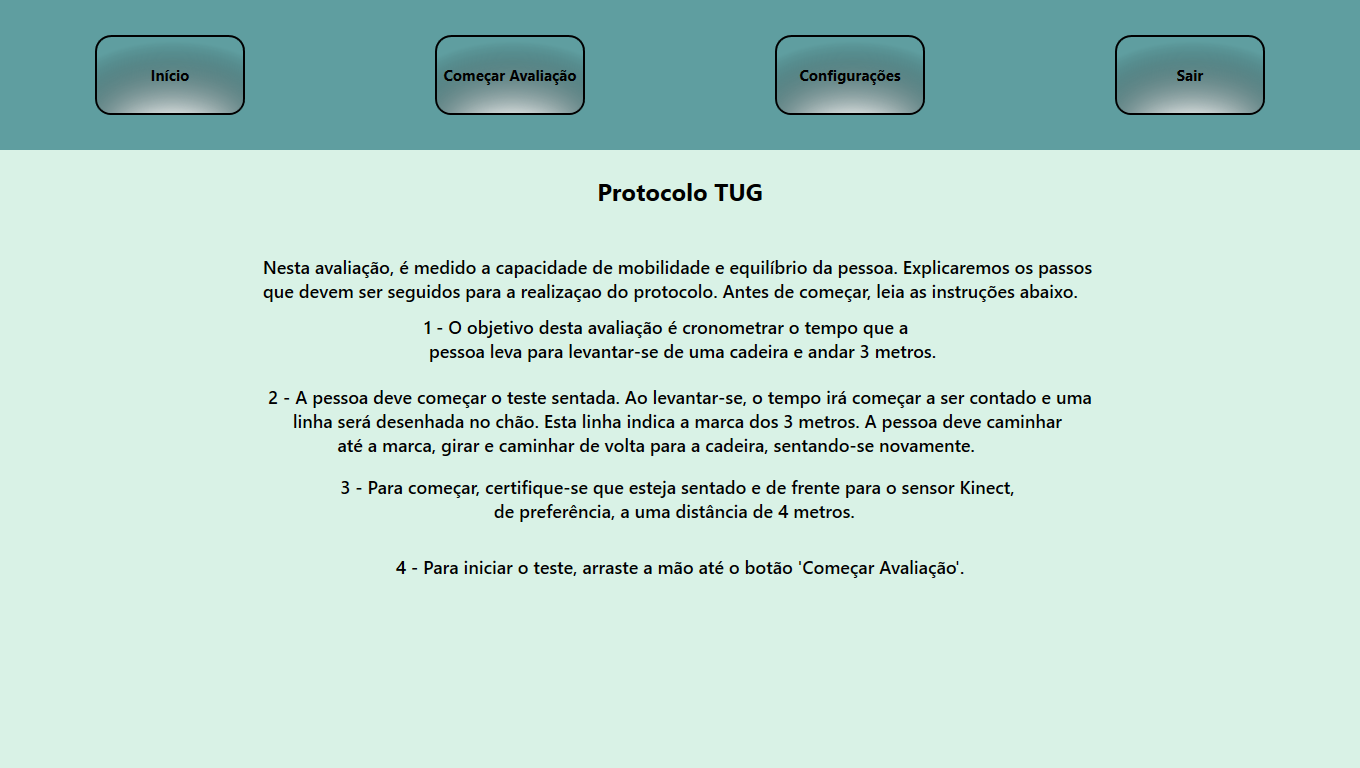
\includegraphics[scale=0.3]{img_1.png}
 \fautor
\end{figure}

\begin{figure}[htb]
\caption{TUG assessment using Kinect}
 \label{fig:img_1e2_kinect}
 \centering
 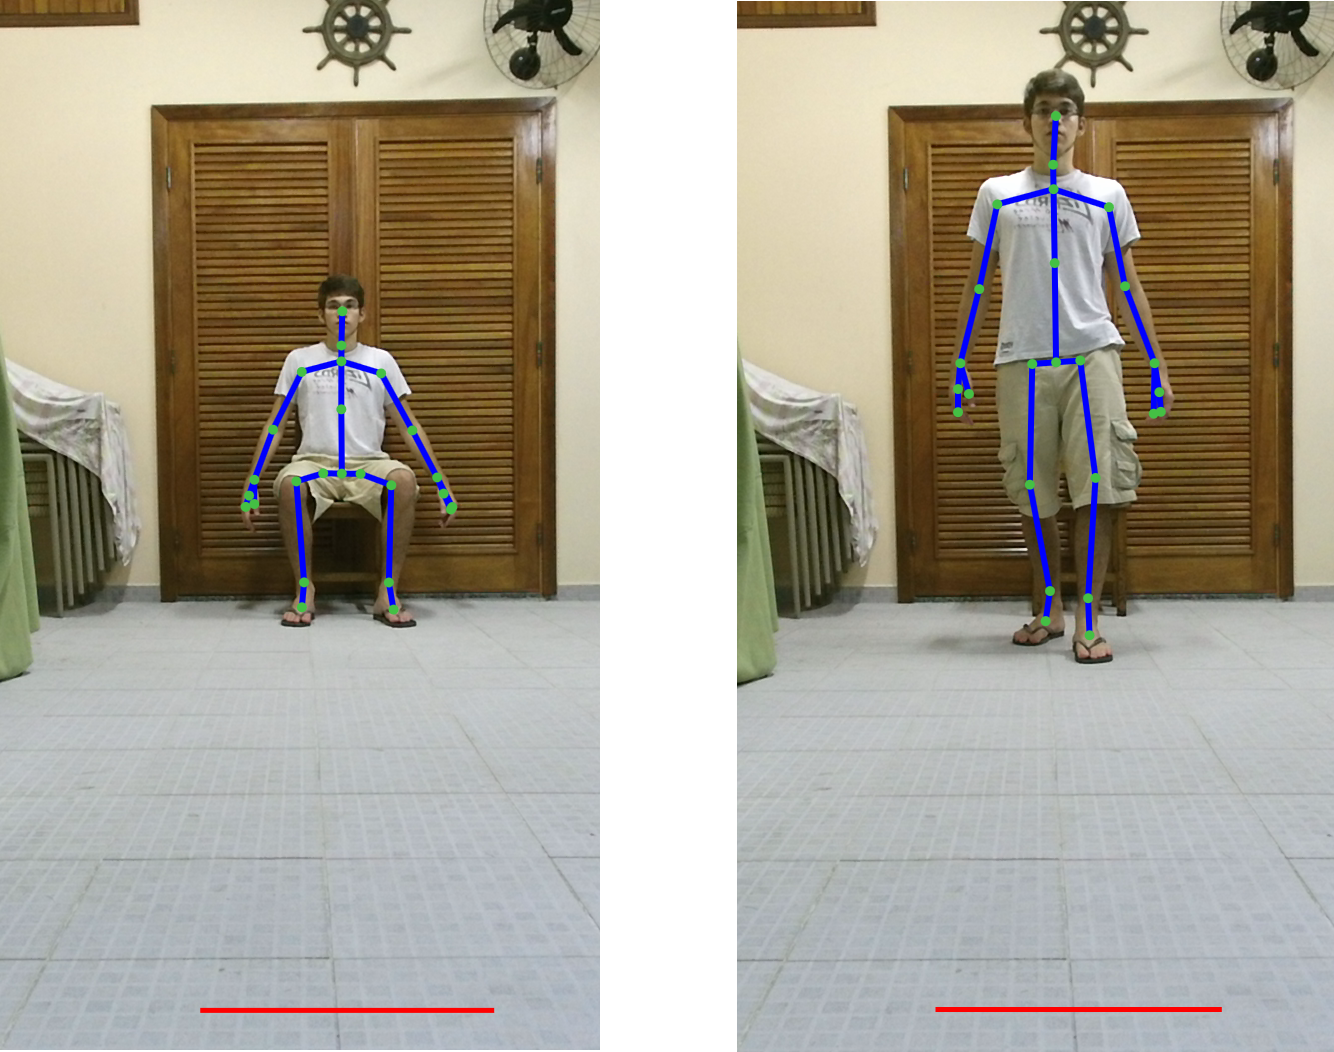
\includegraphics[scale=0.4]{img_2e3.png}
 \fautor
\end{figure}

\begin{figure}[htb]
\caption{Result screen of TUG assessment using Kinect}
 \label{fig:img_3_kinect}
 \centering
 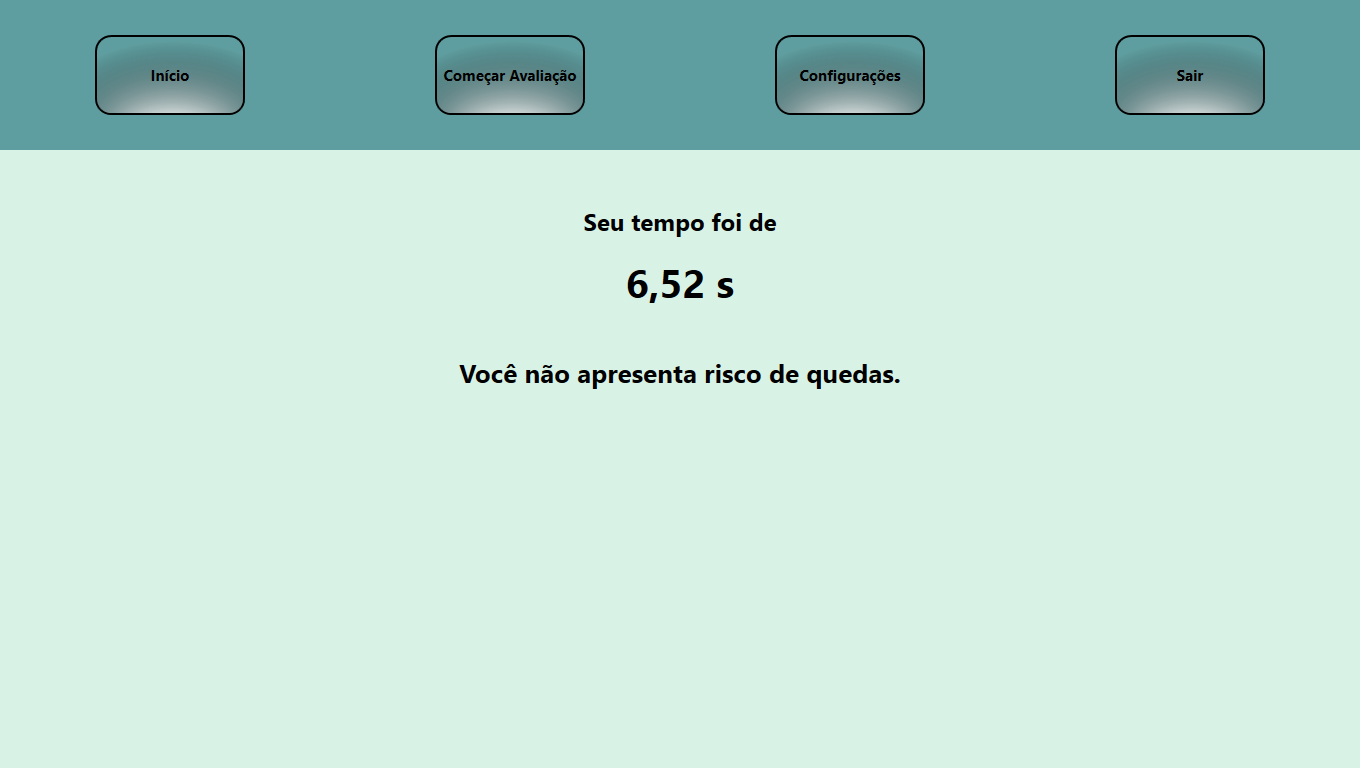
\includegraphics[scale=0.3]{img_4.png}
 \fautor
\end{figure}

%
%\end{apendicesenv}
% ---


\end{document}